\label{cap:Conjuntos}
\chapter{Conjuntos}

\minitoc

El concepto de \textit{conjunto} aparece en todos los campos de las
Matemáticas, pero, ¿qué debe entenderse por él? La \textit{Teoría de conjuntos}
fue introducida por Georg Cantor (1845-1917); desde 1869, Cantor ejerció como
profesor en la Universidad de Halle y entre 1879 y 1884 publicó una serie de
seis artículos en el \textit{Mathematische Annalen}, en los que hizo una
introducción básica a la teoría de conjuntos. En su \textit{Beiträge zur
Begründung der transfiniten Mengenlehre}, Cantor dio la siguiente definición
de conjunto:

\begin{figure}[h]
  \centering
  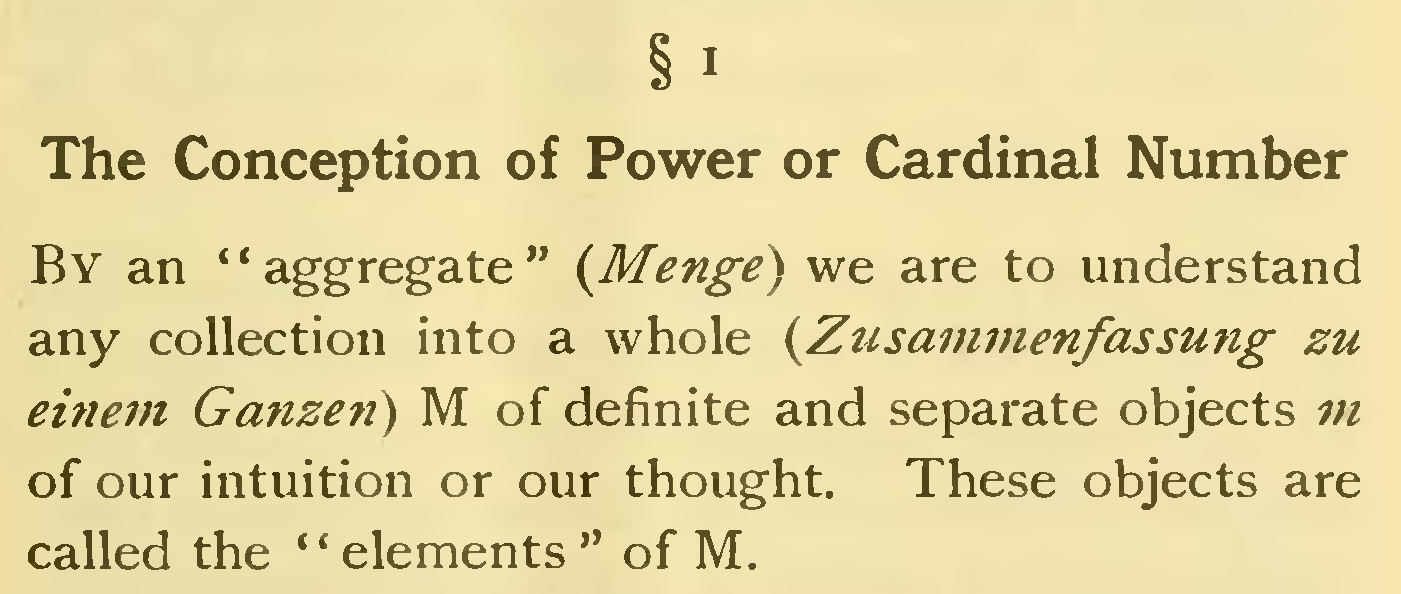
\includegraphics[scale=.2]{fig/definicionConjunto}
  \captionsetup{font=footnotesize}
  \caption{Fragmento del texto traducido al inglés en el que Cantor da la
    definición de conjunto}
\end{figure}

\begin{quote}
  <<Debemos entender por ``conjunto'' (\textit{Menge}) cualquier colección
  vista como un todo (Zusammenfassung zu einem Ganzen), $M$, de objetos
  separados y bien definidos, $m$, de nuestra intuición o pensamiento. Estos
  objetos son los ``elementos'' de $M$>>
\end{quote}

Felix Hausdorff, en 1914, dice: <<un conjunto es una reunión de cosas que
constituyen una totalidad; es decir, una nueva cosa>>, y añade: <<esto puede
difícilmente ser una definición, pero sirve como demostración expresiva del
concepto de conjunto a través de conjuntos sencillos como el conjunto de
habitantes de una ciudad o el de átomos de Hidrógeno del Sol>>.

Un conjunto así definido no tiene que estar compuesto necesariamente de
elementos homogéneos y además, da lugar a cuestiones filosóficas como si
podemos llamar \textit{conjunto} a aquel que no posee ningún elemento.
Matemáticamente, conviene aceptar solo elementos que compartan alguna propiedad
y definir el \textit{conjunto vacío} como aquel que no tiene elemento alguno.

El gran mérito de Cantor fue considerar conjuntos \textit{transfinitos} (que
tiene infinitos elementos), concepto inaudito hasta avanzado el siglo XIX,
hablar del \textit{cardinal} de un conjunto como el número de sus elementos y
hablar de \textit{conjuntos equivalentes} cuando puede establecerse una
biyección entre ellos; ideas ya apuntadas por Bolzano, quien se centró
demasiado en el aspecto filosófico, sin llegar a formalizar sus ideas.\\


A lo largo de la sección, haremos una pequeña introducción a la Teoría de
Conjuntos, presentando formalmente sus conceptos más importantes. A la hora de 
elaborar el contenido se han utilizado los siguientes recursos bibliográficos:

\begin{itemize}
\item el primer tema de la asignatura ``Álgebra básica'' (\cite{Algebra-15a}),
\item los temas de la asignatura ``Informática'' (\cite{Alonso-15a}),
\item el artículo de la Wikipedia ``Set (mathematics)''
  (\cite{Wikipedia-conjuntos} y
\item[$*$] el artículo ``El regalo de Cantor'' (\cite{Regalo-cantor}).
\end{itemize}

\section{El TAD de los conjuntos}

\label{sec:TAD_conjuntos}

En la presente sección, se definen las operaciones básicas necesarias
para trabajar con conjuntos en un lenguaje funcional. En nuestro caso, 
el lenguaje que utilizaremos será Haskell. Daremos la signatura del Tipo
Abstracto de Dato (TAD) de los conjuntos y daremos algunos ejemplos de 
posibles representaciones de conjuntos con las que podríamos trabajar.

A continuación, presentamos las operaciones definidas en el TAD de los 
conjuntos:

\begin{code}
vacio          :: Conj a                         
inserta        :: Eq a => a -> Conj a -> Conj a
elimina        :: Eq a => a -> Conj a -> Conj a
pertenece      :: Eq a => Conj a -> a -> Bool  
esVacio        :: Conj a -> Bool
minimoElemento :: Ord a => Conj a -> a
\end{code}

donde,

\begin{itemize}
\item \texttt{(vacio)} es el conjunto vacío.
\item \texttt{(inserta x c)} es el conjunto obtenido añadiendo el      
      elemento \texttt{x} al conjunto \texttt{c}.
\item \texttt{(elimina x c)} es el conjunto obtenido eliminando el
      elemento \texttt{x} del conjunto \texttt{c}.
\item \texttt{(pertenece x c)} se verifica si \texttt{x} pertenece al
      conjunto \texttt{c}.
\item \texttt{(esVacio c)} se verifica si \texttt{c} no tiene ningún
      elemento.
\item \texttt{(minimoElemento c)} devuelve el mínimo elemento del      
      conjunto \texttt{c}.\\
\end{itemize}


Hemos de tener en cuenta que a la hora de crear un nuevo tipo de dato 
con el que representar a los conjuntos, este debe ser compatible con 
la entidad matemática que representa.\\

Estas son algunas de las posibles representaciones con las que podríamos
trabajar con conjuntos en Haskell:

\begin{itemize}
\item En primer lugar, podemos trabajar con la librería \texttt{Data.Set}; en
  este caso, la implementación del tipo de dato \texttt{Set} está basado en
  árboles binarios balanceados.
\item Por otra parte, podemos definir un nuevo tipo \texttt{Cj xs} con el que
  trabajar con conjuntos como listas no ordenadas con duplicados, como listas
  no ordenadas sin duplicados o como listas ordenadas sin duplicados.
\item Otra opción sería trabajar directamente con conjuntos como listas; para
  ello, debemos ignorar las repeticiones y el orden con vista a la igualdad de
  conjuntos. 
\item Los conjuntos que sólo contienen números (de tipo \texttt{Int)} entre
  $0$ y $n-1$, se pueden representar como números binarios con $n$ bits donde
  el bit $i (0 ≤ i < n)$ es $1$ syss el número $i$ pertenece al conjunto.
\end{itemize}

\begin{nota}
  Las funciones que aparecen en la especificación del TAD no dependen 
  de la representación que elijamos.
\end{nota}

\section{Representaciones de conjuntos}

\label{sec:rep_conjuntos}


\comentario{Exportar en cada una de las distintas representaciones de conjuntos
  todas las operaciones de forma que se pueda elegir cualquiera de ellas.}

\subsection{Conjuntos como listas ordenadas sin repetición}

\entrada{ConjuntosConListasOrdenadasSinRepeticion}

\subsection{Conjuntos como listas sin repetición}

\entrada{ConjuntosConListas}

\section{Elección de la representación de conjuntos}

\begin{nota}
En el módulo \texttt{Conjuntos} se elige la representación de conjunto con la
que se trabajará.
\end{nota}

\entrada{Conjuntos}
